



\chapter{Ensembles de nombres}

\section{Différents types de nombres}

\subsection{Notations}

\begin{Définition} $ $ \\
\begin{center}
\renewcommand{\arraystretch}{2}
\begin{tabular}{|c|c|C{3.5cm}|c|}
\hline 
\textbf{Ensembles de nombres} & \textbf{Notation} & \textbf{Définition} & \textbf{Exemples} \\
\hline 
Nombres \textbf{entiers naturels} & $\N$ &  Nombres entiers positifs ou nuls  &
 \\ 
\hline 
Nombres \textbf{entiers relatifs} & $\Z$ &  Nombres entiers positifs ou négatifs ou nuls  &  \\ 
\hline 
Nombres \textbf{décimaux} & $\D$ &  Nombres de la forme $\dfrac{a}{10^n}$, $a \in \Z$ et $n \in \N$  &  \phantom{$-2,1=-\dfrac{21}{10} \text{ }$ ; $\dfrac{2}{5}=\dfrac{4}{10}$ ; $5=\dfrac{5}{1}$} \\ 
\hline 
Nombres \textbf{rationnels} & $\Q$ & Nombres de la forme $\dfrac{a}{b}$, $a \in \Z$ et $b \in \N$, $b \neq 0$ &  \\ 
\hline 
Nombres \textbf{réels} & $\R$ & Tous les nombres connus en 2nde  & \phantom{$5$ ; $-8$ ; $-2,1=-\dfrac{21}{10}$ ; $\dfrac{1}{3}$ ; $\sqrt{2}$ ; $ \pi $ } \\ 
\hline 
\end{tabular} 
\end{center}
\end{Définition}

\begin{Propriété}
Un nombre rationnel est caractérisé soit par une écriture décimale ayant un nombre fini de décimales, soit par une écriture décimale comportant une suite de chiffres qui se répète (période).
\end{Propriété}

\begin{Exemple}
\leavevmode\vspace{-\baselineskip}
\begin{itemize}[label=\textcolor{Couleur10}{$\bullet$}]
\item 0,125 est un nombre \ligne

\item $\dfrac{127}{11} = 11,545454...$ est un nombre \ligne

\end{itemize}
\end{Exemple}

\newpage

\subsection{Inclusions}

\begin{Propriété} $ $\\
\begin{itemize}[label=\textcolor{Couleur2}{$\bullet$}]
\item $\N$ est inclus dans $\Z$ : $\N \subset \Z$
\item $\Z$ est inclus dans $\D$ : $\Z \subset \D$
\item $\D$ est inclus dans $\Q$ : $\D \subset \Q$
\item $\Q$ est inclus dans $\R$ : $\Q \subset \R$
\end{itemize}
Ou encore :
\begin{center}
$\N \subset \Z \subset \D \subset \Q \subset \R$
\end{center}

\begin{center}
\begin{minipage}[c]{0.6\linewidth}
\begin{center} 
\begin{tikzpicture}[scale=.75] 
\def\R{ (-1,0) rectangle (10,6) };
\def\Q{ (-0.8,0.2) rectangle (8,5) };
\def\D{ (-0.6,0.4) rectangle (6,4) };
\def\Z{ (-0.4,0.6) rectangle (4,3) };
\def\N{ (-0.2,0.8) rectangle (2,2) };




\begin{scope}
\clip \R ;
\fill[Couleur7!20] \R ;
\end{scope}

\begin{scope}
\clip \R ;
\fill[orange!20] \Q;
\end{scope}

\begin{scope}
\clip \Q ;
\fill[YellowGreen!20] \D;
\end{scope}

\begin{scope}
\clip \D ;
\fill[pink!20] \Z;
\end{scope}

\begin{scope}
\clip \Z ;
\fill[violet!20] \N;
\end{scope}

\draw[Couleur7] \R ;
\draw[orange] \Q ;
\draw[YellowGreen] \D ;
\draw[pink!75!black] \Z ;
\draw[violet] \N ;

\draw[Couleur7] (9.7,5.7) node{$\mathbb{R}$} ; 
\draw[orange] (7.7,4.7) node{$\mathbb{Q}$} ; 
\draw[YellowGreen] (5.7,3.7) node{$\mathbb{D}$} ; 
\draw[pink!75!black] (3.7,2.7) node{$\mathbb{Z}$} ; 
\draw[violet] (1.7,1.7) node{$\mathbb{N}$} ; 


\draw (0.4,1.6) node{$5$} ; 
\draw (1.3,1.1) node{$258$} ; 
\draw (3,1.2) node{$-3$} ; 
\draw (1.1,2.5) node{$-24$} ; 
\draw (3.4,3.5) node{$0,01$} ; 
\draw (1,3.5) node{$-2,1$} ; 
\draw (4.8,1.9) node{$\dfrac{3}{4}$} ; 
\draw (7.4,1.4) node{$\dfrac{1}{3}$} ; 
\draw (6.8,3.8) node{$-\dfrac{5}{6}$} ; 
\draw (5,5.4) node{$-\pi$} ; 
\draw (8.9,2) node{$-\sqrt{2}$} ; 

\end{tikzpicture} 
\end{center}
\end{minipage}
\end{center}
\end{Propriété}

\section{Intervalles}

\subsection{Intervalles de $\R$}

\begin{Définition}
Soit $a$ et $b$ deux nombres réels tels que $a<b$.

\begin{multicols}{2}
\begin{center}
\begin{tabular}{|>{\centering\arraybackslash}m{2cm}|>{\centering\arraybackslash}m{3cm}|>{\centering\arraybackslash}m{2cm}|}
\hline 
 Ensembles des réels $x$ tels que & Réprésentation sur une droite graduée & Intervalles bornées  \\
\hline   
$a {\color{Couleur1}{\leq}} x   {\color{violet}{\leq}} b $ & 
\begin{tikzpicture}
\draw[gray] (0,0) -- (2,0);
\draw[-stealth]|-(2,0)node[above]{};
\foreach \x/\xtext in {0.5/a,1.5/b} {
\draw (\x,0.1cm) -- (\x,-0.1cm) node[below] {$\xtext\strut$}; };    \node[Couleur7, thick] at (0.5,0) {${\big[}$};
    \node[violet, thick] at (1.5,0) {${\big]}$};
   \draw[orange!70, thick] (0.5,0) -- (1.5,0);
\end{tikzpicture}
 & ${\color{Couleur1}{\big[}} a \mathpunct{} ; b {\color{violet}{\big]}} $ \\
 \hline
 $a {\color{YellowGreen}{<}} x   {\color{Couleur10}{<}} b $ & 
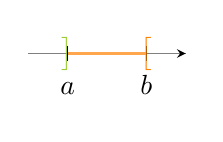
\begin{tikzpicture}
\draw[gray] (0,0) -- (2,0);
\draw[-stealth]|-(2,0)node[above]{};
\foreach \x/\xtext in {0.5/a,1.5/b} {
\draw (\x,0.1cm) -- (\x,-0.1cm) node[below] {$\xtext\strut$}; };    \node[YellowGreen, thick] at (0.5,0) {${\big]}$};
    \node[orange, thick] at (1.5,0) {${\big[}$};
   \draw[orange!70, thick] (0.5,0) -- (1.5,0);
\end{tikzpicture}
 & ${\color{YellowGreen}{\big]}} a \mathpunct{} ; b {\color{Couleur10}{\big[}} $ \\
 \hline
  $a {\color{Couleur1}{\leq}} x   {\color{Couleur10}{<}} b $ & 
\begin{tikzpicture}
\draw[gray] (0,0) -- (2,0);
\draw[-stealth]|-(2,0)node[above]{};
\foreach \x/\xtext in {0.5/a,1.5/b} {
\draw (\x,0.1cm) -- (\x,-0.1cm) node[below] {$\xtext\strut$}; };    \node[Couleur7, thick] at (0.5,0) {${\big[}$};
    \node[orange, thick] at (1.5,0) {${\big[}$};
   \draw[orange!70, thick] (0.5,0) -- (1.5,0);
\end{tikzpicture}
 & ${\color{Couleur1}{\big[}} a \mathpunct{} ; b {\color{Couleur10}{\big[}} $ \\
 \hline
  $a {\color{YellowGreen}{<}} x   {\color{violet}{\leq}} b $ & 
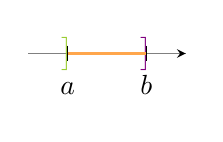
\begin{tikzpicture}
\draw[gray] (0,0) -- (2,0);
\draw[-stealth]|-(2,0)node[above]{};
\foreach \x/\xtext in {0.5/a,1.5/b} {
\draw (\x,0.1cm) -- (\x,-0.1cm) node[below] {$\xtext\strut$}; };    \node[YellowGreen, thick] at (0.5,0) {${\big]}$};
    \node[violet, thick] at (1.5,0) {${\big]}$};
   \draw[orange!70, thick] (0.5,0) -- (1.5,0);
\end{tikzpicture}
 & ${\color{YellowGreen}{\big]}} a \mathpunct{} ; b {\color{violet}{\big]}} $ \\
 \hline

 

\end{tabular}
\end{center}
\columnbreak
\begin{center}
\begin{tabular}{|>{\centering\arraybackslash}m{2cm}|>{\centering\arraybackslash}m{3cm}|>{\centering\arraybackslash}m{2cm}|}
\hline 
 Ensembles des réels $x$ tels que & Réprésentation sur une droite graduée & Intervalles non bornées  \\
\hline   
$a {\color{Couleur1}{\leq}} x   $ & 
\begin{tikzpicture}
\draw[gray] (0,0) -- (2,0);
\draw[-stealth]|-(2.1,0)node[above]{};
\foreach \x/\xtext in {1/a,} {
\draw (\x,0.1cm) -- (\x,-0.1cm) node[below] {$\xtext\strut$}; };    \node[Couleur7, thick] at (1,0) {${\big[}$};
   \draw[orange!70, thick] (1,0) -- (2,0);
\end{tikzpicture}
 & ${\color{Couleur1}{\big[}} a \mathpunct{} ; +\infty {\color{black}{\big[}} $ \\
 \hline
 $a {\color{YellowGreen}{<}} x   $ & 
\begin{tikzpicture}
\draw[gray] (0,0) -- (2,0);
\draw[-stealth]|-(2.1,0)node[above]{};
\foreach \x/\xtext in {1/a,} {
\draw (\x,0.1cm) -- (\x,-0.1cm) node[below] {$\xtext\strut$}; };    \node[YellowGreen, thick] at (1,0) {${\big]}$};
   \draw[orange!70, thick] (1,0) -- (2,0);
\end{tikzpicture}
 & ${\color{YellowGreen}{\big]}} a \mathpunct{} ; +\infty {\color{black}{\big[}}$ \\
 \hline
  $ x   {\color{violet}{\leq}} b $ & 
\begin{tikzpicture}
\draw[gray] (0,0) -- (2,0);
\draw[-stealth]|-(2,0)node[above]{};
\foreach \x/\xtext in {1/b} {
\draw (\x,0.1cm) -- (\x,-0.1cm) node[below] {$\xtext\strut$}; };    \node[violet, thick] at (1,0) {${\big]}$};

   \draw[orange!70, thick] (0,0) -- (1,0);
\end{tikzpicture}
 & ${\color{black}{\big]}} -\infty \mathpunct{} ; b {\color{violet}{\big]}} $ \\
 \hline
  $ x   {\color{Couleur10}{<}} b $ & 
\begin{tikzpicture}
\draw[gray] (0,0) -- (2,0);
\draw[-stealth]|-(2,0)node[above]{};
\foreach \x/\xtext in {1/b} {
\draw (\x,0.1cm) -- (\x,-0.1cm) node[below] {$\xtext\strut$}; };    \node[orange, thick] at (1,0) {${\big[}$};

   \draw[orange!70, thick] (0,0) -- (1,0);
\end{tikzpicture}
 & ${\color{black}{\big]}} -\infty \mathpunct{} ; b {\color{Couleur10}{\big[}} $ \\
 \hline

 

\end{tabular}
\end{center}
\end{multicols}

\end{Définition}

\begin{Remarque} 
\vspace{-0.5cm}
\begin{itemize}[label=\textcolor{Couleur7}{$\bullet$}]
\item Avec l'infini ($\infty$), le crochet est toujours "ouvert".
\item $1 \in \left[ -2 ; 3\right ]$
\item $4 \notin \left[ -2 ; 3\right ]$
\item $1 \notin \left[ -2 ; 1\right [$
\end{itemize}
\end{Remarque}


\newpage


\begin{Remarque}
Voici quelques notations très utiles.
\begin{multicols}{5}
\item $]-\infty \mathpunct{} ; +\infty [ =\R$
\item $ [ 0 \mathpunct{} ; +\infty [ = \R^+$
\item $]-\infty \mathpunct{} ; 0 ] =\R^-$
\item $ ] 0 \mathpunct{} ; +\infty [ = \R^{\ast+}$
\item $]-\infty \mathpunct{} ; 0 [ =\R^{\ast-}$
\end{multicols}
\end{Remarque}

\subsection{Réunion et intersection d'intervalles}

\begin{Définition}
{\bf{L'intersection}} de deux intervalles est l'ensemble des réels qui appartiennent à l'un {\bf{et}} l'autre des intervalles. \\
On la note $\cap$ .
\end{Définition}

\begin{Exemples} 
\leavevmode\vspace{-\baselineskip}
\vspace{-0.5cm}
\setlength{\columnsep}{2cm}
\begin{multicols}{2}
\begin{itemize}[label=\textcolor{Couleur10}{$\bullet$}]
\item $]-\infty\mathpunct{} ;5]\cap[2\mathpunct{} ;6]=$ \pointille{5cm}
\item $]-\infty\mathpunct{} ;5]\cap]2\mathpunct{} ;6]=$ \pointille{5cm}
\item $[-3\mathpunct{} ;4]\cap[4\mathpunct{} ;6]=$ \pointille{5cm}
\item $[12\mathpunct{} ;56]\cap[-3\mathpunct{} ;0]=$ \pointille{5cm}
\end{itemize}
\end{multicols}
\end{Exemples}

\begin{Définition}
{\bf{La réunion}} de deux intervalles est l'ensemble des réels qui appartiennent à l'un {\bf{ou}} l'autre des intervalles. \\
On la note $\cup$ .
\end{Définition}

\begin{Exemples}
\leavevmode\vspace{-\baselineskip}
\vspace{-0.5cm}
\setlength{\columnsep}{2cm}
\begin{multicols}{2}
\begin{itemize}[label=\textcolor{Couleur10}{$\bullet$}]
\item $[-3\mathpunct{} ;4]\cup[4\mathpunct{} ;6]=$ \pointille{5cm}
\item $]-\infty\mathpunct{} ;5]\cup[4\mathpunct{} ;10]=$ \pointille{5cm}
\item $]-\infty\mathpunct{} ;1[\cup]1\mathpunct{} ;+\infty[=$ \pointille{5cm}
\item  $]-\infty\mathpunct{} ;0[\cup]0\mathpunct{} ;+\infty[=$ \pointille{5cm}
\end{itemize}
\end{multicols}
\end{Exemples}

\begin{minipage}[c]{0.3\linewidth}
\begin{center} 
\begin{tikzpicture}[scale=.4] 
\def\A{(2,2) circle[x radius=2cm, y radius=1.2cm, rotate=40]} ;
\def\B{(4,2) circle[x radius=1.5cm, y radius=1cm, rotate=-20]} ;

\begin{scope}
\clip \A ;
\fill[Couleur7] \B;
\end{scope}

\draw \A ;
\draw (0.7,3.3) node{$A$} ; \draw \B ;
\draw (4.5,0.4) node{$B$} ; 
\draw[Couleur7] (5,3.5) node{$A\cap B$} ; 
\end{tikzpicture} 
\end{center}
\end{minipage} \hfill
\begin{minipage}[c]{0.3\linewidth}
\begin{center} 
\begin{tikzpicture}[scale=.4] 
\def\C{ (0,0) rectangle (6,4) };
\def\A{(2,2) circle[x radius=2cm, y radius=1.2cm, rotate=40]} ;
\def\B{(4,2) circle[x radius=1.5cm, y radius=1cm, rotate=-20]} ;

\begin{scope}
\clip \A ;
\fill[Couleur10!90] \B ;
\end{scope}

\begin{scope}
\clip \A ;
\fill[Couleur10!90] \B \C;
\end{scope}

\begin{scope}
\clip \B ;
\fill[Couleur10!90] \A \C;
\end{scope}

\draw \A ;
\draw (0.7,3.3) node{$A$} ; \draw \B ;
\draw (4.5,0.4) node{$B$} ; 
\draw[Couleur10] (5,3.5) node{$A\cup B$} ; 
\end{tikzpicture} 
\end{center}
\end{minipage}\hfill
\begin{minipage}[c]{0.3\linewidth}
\begin{center} 
\begin{tikzpicture}[scale=.4] 
\def\C{ (0,0) rectangle (6,4) };
\def\A{(2,2) circle[x radius=2cm, y radius=1.2cm, rotate=40]} ;
\def\B{(4,2) circle[x radius=1.5cm, y radius=1cm, rotate=-20]} ;

\begin{scope}
\clip \A ;
\fill[Couleur6] \B \C;
\end{scope}

\draw \A ;
\draw (0.7,3.3) node{$A$} ; \draw \B ;
\draw (4.5,0.4) node{$B$} ; 
\draw[Couleur6] (5,3.5) node{$A\setminus B$} ; 
\end{tikzpicture} 
\end{center}
\end{minipage}

\section{Puissances, notation scientifique et arrondis}

\subsection{Puissances}

\begin{Définition} $ $\\
\begin{itemize}[label=\textcolor{Couleur6}{$\bullet$}]
\item  Soit $a$ un nombre réel et $n\in \Z$, $n\geq 2$. \\
Le produit $\underbrace{a\times ...\times a}_{n \text{ facteurs}}$  est une puissance de $a$. On la nomme $a$ puissance $n$ ou $a$ exposant $n$ et il se note : $$\underbrace{a\times ...\times a}_{n \text{ facteurs}}= a^n$$ \\
\underline{Cas particuliers} : $\quad\quad{\color{Couleur6}{\bullet}}\quad a^0=1$ avec $(a\neq 0)$ $\quad\quad\quad\quad$ ${\color{Couleur6}{\bullet}} \quad a^1=a$
\vspace{0.5cm}
\item Soit $a$ un nombre réel non nul $(a\neq 0)$ et $n$ un nombre entier.\\
$a^{-n}$ désigne l'inverse de $a^n$ et donc :
$$a^{-n}=\dfrac{1}{a^n}$$
\underline{Cas particulier} : $\quad a^{-1}=\dfrac{1}{a^1}=\dfrac{1}{a}$. C'est donc l'inverse de $a$.
\end{itemize}
\end{Définition}

\newpage

\begin{Exemples}

\vspace{-0.5cm}
\begin{multicols}{2}
\begin{itemize}[label=\textcolor{Couleur10}{$\bullet$}]
\item $3^4=$ \ligne

\item $(-2)^3=$ \ligne

\item $(-12)^2=$ \ligne

\item $10^5=$ \ligne

\item $2^{-4}=$ \ligne

\item $(-5)^{-2}=$ \ligne

\item $10^{-3}=$ \ligne

\end{itemize}
\end{multicols}
\end{Exemples}

\begin{Propriété}
Soit $a,b$ des réels différents de zéro $(a,b \in \R^\ast)$ et $m,n$ des entiers relatifs$(m,n \in \Z)$ alors : 
\vspace{-0.5cm}
\begin{multicols}{2}
\begin{itemize}[label=\textcolor{Couleur2}{$\bullet$}]
\item $a^m\times a^n=a^{m+n}$
\item $\dfrac{a^m}{a^n}=a^{m-n}$
\item $(a\times b)^n=a^n\times b^n$
\item $(a^m)^n=a^{m\times n}$
\end{itemize}
\end{multicols}
\end{Propriété}

\begin{Exemples}
\leavevmode\vspace{-\baselineskip}
\vspace{-0.5cm}
\begin{multicols}{2}
\begin{itemize}[label=\textcolor{Couleur10}{$\bullet$}]
\item $3^2\times 3^3=$ \ligne

\item $\dfrac{10^3}{10^2}=$ \ligne

\item $(2\times x)^{3}=$ \ligne

\item $(10^3)^2=$ \ligne

\item $5^6\times 9^6=$ \ligne

\end{itemize}
\end{multicols}
\end{Exemples}

\begin{Remarque}
\leavevmode\vspace{-\baselineskip}
\vspace{-0.3cm}
\begin{multicols}{2}
\begin{itemize}[label=\textcolor{Couleur7}{$\bullet$}]
\item $(3x)^2=(3x)\times (3x)=3^2\times x^2=9x^2$
\item $3x^2=3\times x\times x$
\item $(-x)^2=(-x)\times (-x)=(-1)^2\times x^2=x^2$
\item $-x^2=-(x\times x)$
\end{itemize}
\end{multicols}
\end{Remarque}

\subsection{Notation scientifique}

\begin{Définition}
La notation scientifique d'un nombre décimal différent de zéro est l'unique écriture de la forme : 
$$\pm a\times 10^n \text{ avec } \left\{
    \begin{array}{ll}
       1\leq a <  10  & \\
      n\in \Z  & 
    \end{array}
\right.
$$
\end{Définition}

\begin{Exemples}
\leavevmode\vspace{-\baselineskip}
\vspace{-0.7cm}
\begin{multicols}{2}
\begin{itemize}[label=\textcolor{Couleur10}{$\bullet$}]
\item $823 951=$ \ligne
\item $-10 500=$ \ligne
\item $0, 123 456=$ \ligne
\item $-0,000 123=$ \ligne
\end{itemize}
\end{multicols}
\end{Exemples}



\section{Équations et inéquations}

\subsection{Équations de degré 1}

\begin{Définition}
Une \textbf{équation d'inconnue $x$} est une \textbf{égalité} qui peut être vraie pour certaines valeurs de $x$ et fausse pour d'autres.\\
\textbf{Résoudre dans $\R$ une équation} d'inconnue $x$, c'est trouver toutes les valeurs possibles de $x$ telles que l'égalité soit vérifiée. 
On détermine ainsi \textbf{l'ensemble des solutions} (noté $S$).
\end{Définition}
\newpage
\begin{Exemples}
Résoudre dans $\R$ les équations suivantes : \\
\vspace{-0.5cm}
\begin{multicols}{3}
\begin{center}
$ 3 + x = -7$
\end{center}

 \columnbreak
\begin{center}

$-4x=7$ 
\end{center}

 \columnbreak

\begin{center}
$3x+7=5(x - 4)$
\end{center}
\end{multicols}
\vspace{-0.5cm}
\ligne

\ligne

\ligne

\ligne

\ligne

\ligne

\end{Exemples}

\subsection{Inégalités}

\begin{Propriété}
Soient $a,b,$ et $c$ des réels,
\begin{itemize}[label=\textcolor{Couleur2}{$\bullet$}]
\item Si $a\leq b$ {\textcolor{Couleur1}{(respectivement $a\geq b$)}} alors $a{\color{Couleur10}{+c}} \leq b{\color{Couleur10}{+c}}$ {\textcolor{Couleur1}{(respectivement $a{\color{Couleur10}{+c}} \geq b{\color{Couleur10}{+c}}$)}}.
\item  Si $a\leq b$ {\textcolor{Couleur1}{(respectivement $a\geq b$)}} alors $a{\color{Couleur10}{-c}} \leq b{\color{Couleur10}{-c}}$ {\textcolor{Couleur1}{(respectivement $a{\color{Couleur10}{-c} }\geq b{\color{Couleur10}{-c}}$)}}.
\end{itemize}
Autrement dit, si on ajoute ou soustrait un même nombre aux deux membres d'une inégalité, on ne change pas l'ordre de cette inégalité.
\end{Propriété}

\begin{Exemple}
$4\leq 7$ alors \ligne
\end{Exemple}

\begin{Propriété}
Soient $a,b,$ et $c$ des réels,
{\begin{center}
\begin{tabular}{|>{\centering\arraybackslash}m{2cm}|>{\centering\arraybackslash}m{3cm}|>{\centering\arraybackslash}m{3cm}|}
\hline
 & $c{\color{Couleur10}{>0}}$ & \hspace{-0.7cm} $\quad  c{\color{Couleur10}{<0}}$ \\ 
 \hline
 $a\leq b$ 
 & {$$\begin{aligned}
  a{\color{Couleur1}{\times c }}&\leq b{\color{Couleur1}{\times c }} \\
  \dfrac{a}{{\color{Couleur1}{ c }}}&\leq\dfrac{b}{{\color{Couleur1}{ c }}}
 \end{aligned}$$} 
 & {$$\begin{aligned}
a{\color{Couleur1}{\times c }}&{\color{Couleur10}{\geq }} b{\color{Couleur1}{\times c }}\\
\dfrac{a}{{\color{Couleur1}{ c }}}&{\color{Couleur10}{\geq }}\dfrac{b}{{\color{Couleur1}{ c }}}
 \end{aligned}$$} \\
 \hline
 $a\geq b$ 
 &{$$\begin{aligned}
  a{\color{Couleur1}{\times c }}&\geq b{\color{Couleur1}{\times c }} \\
  \dfrac{a}{{\color{Couleur1}{ c }}}&\geq\dfrac{b}{{\color{Couleur1}{ c }}}
 \end{aligned}$$} 
 & {$$\begin{aligned}
a{\color{Couleur1}{\times c }}&{\color{Couleur10}{\leq }} b{\color{Couleur1}{\times c }}\\
\dfrac{a}{{\color{Couleur1}{ c }}}&{\color{Couleur10}{\leq }}\dfrac{b}{{\color{Couleur1}{ c }}}
 \end{aligned} $$}\\
 \hline
\end{tabular}
\end{center}}

Autrement dit, 
\begin{itemize}[label=\textcolor{Couleur2}{$\bullet$}]
\item Si on multiplie ou divise les deux membres d'une inégalité par un même nombre positif on ne change pas l'ordre de cette inégalité.
\item Si on multiplie ou divise les deux membres d'une inégalité par un même nombre négatif \textbf{on change l'ordre} de l'inégalité.
\end{itemize}
\end{Propriété}
\newpage
\begin{Exemple}
\leavevmode\vspace{-\baselineskip}
\begin{itemize}
\item $7\geq4$ \ligne
\item $7\geq 4$ \ligne
\end{itemize}
\end{Exemple}

\begin{Propriété}
Soient $a,b,c$ et $d$ quatre réels. 
\begin{itemize}[label=\textcolor{Couleur2}{$\bullet$}]
\item Si $a\leq b$ et $c\leq d$ alors $a+c\leq b+d$.
\item Si $a\geq b$ et $c\geq d$ alors $a+c\geq b+d$.
\end{itemize}
\end{Propriété}

\begin{Remarque}
Toutes ces propriétés restent vraies avec des inégalités strictes ($>,<$).
\end{Remarque}

\vspace{0.5cm}

\subsection{Inéquations}

\begin{Définition}
Une \textbf{inéquation d'inconnue $x$} est une \textbf{inégalité} qui peut être vraie pour certaines valeurs de $x$
et fausse pour d'autres.
\textbf{Résoudre dans $\R$ une inéquation} d'inconnue $x$, c'est trouver toutes les valeurs possibles de
$x$ telles que l'inégalité soit vérifiée.
On détermine ainsi \textbf{l'ensemble des solutions} (noté $S$).
\end{Définition}

\begin{Exemple}
\begin{center}
\begin{tabular}{C{8.5cm}|C{8.5cm}} \arrayrulecolor{Couleur10}
Résoudre dans $\R$ : $4x+5\leq 21$ & Résoudre dans $\R$ : $-5x+7< 28$ \\
\ligne  & \ligne  \\
\ligne  & \ligne  \\
\ligne  & \ligne  \\
\ligne  & \ligne  \\
\ligne  & \ligne  \\
\ligne  & \ligne  \\
\ligne  & \ligne  \\
\ligne  & \ligne  \\
\ligne  & \ligne  \\

\end{tabular}
\end{center}

\end{Exemple}

\bigskip

\newpage

\section*{Exercices - Ensembles de nombres}
\addcontentsline{toc}{section}{Exercices}
{\setlength{\columnseprule}{0pt}
\setcounter{NumEx}{1}

\subsection*{Différents types de nombres}


\begin{Exercice} Pour chaque nombre, cocher le ou les ensembles auxquels il appartient.
\begin{center}
\renewcommand{\arraystretch}{2.5}
\begin{tabular}{|>{\centering\arraybackslash}p{2 cm}|>{\centering\arraybackslash}p{2 cm}|>{\centering\arraybackslash}p{2 cm}|>{\centering\arraybackslash}p{2 cm}|>{\centering\arraybackslash}p{2 cm}|>{\centering\arraybackslash}p{2 cm}|}
\arrayrulecolor{Couleur6}\hline 
 & $\mathbb{N}$ & $\mathbb{Z}$ & $\mathbb{D}$ & $\mathbb{Q}$ & $\mathbb{R}$ \\ 
\hline 
3 &  &  &  &  &  \\ 
\hline 
$-2$ &  &  &  &  &  \\ 
\hline 
$\dfrac{1}{2}$ &  &  &  &  &  \\ 
\hline 
$\dfrac{1}{3}$ &  &  &  &  &  \\ 
\hline 
$5,67$ &  &  &  &  &  \\ 
\hline 
$\sqrt{2}$ &  &  &  &  &  \\ 
\hline 
$\sqrt{36}$ &  &  &  &  &  \\ 
\hline 
$-\dfrac{37}{5}$ &  &  &  &  &  \\ 
\hline 
$\dfrac{138}{22}$ &  &  &  &  &  \\ 
\hline 
$4$ &  &  &  &  &  \\ 
\hline 
$-\dfrac{1}{4}$ &  &  &  &  &  \\ 
\hline 
$(-5)^2$ &  &  &  &  &  \\ 
\hline 
$\sqrt{5}$ &  &  &  &  &  \\ 
\hline 
$\sqrt{7}^3$ &  &  &  &  &  \\ 
\hline 
$\pi$ &  &  &  &  &  \\ 
\hline 
$\dfrac{\sqrt{121}}{11}$ &  &  &  &  &  \\ 
\hline 
$\dfrac{10}{5}$ &  &  &  &  &  \\ 
\hline 
\end{tabular} 
\end{center}
\end{Exercice}

\newpage

\begin{Exercice}  Compléter par l'un des symboles : $\in$ ou $\notin$.

\begin{multicols}{3}
\begin{enumerate}
\item $2$ ... $\left[ 0 ; 9 \right]$ 
\item $-2$ ... $\left[ 1 ; 7 \right[$
\item $3$ ... $\left[ 3 ; 5 \right[$  
\item $12$ ... $\left[ 11 ; 12 \right[$
\item $8$ ... $\left] 1 ; 8 \right[$
\item $\sqrt{25}$ ... $\mathbb{N}$ 
\item $-7,5$ ... $\mathbb{Z}$ 
\item $\dfrac{13}{4}$ ... $\mathbb{Q}$   
\item $-\dfrac{\sqrt{144}}{2}$ ... $\mathbb{Z}$  
\end{enumerate}
\end{multicols} 

\end{Exercice}

\begin{Exercice}  Compléter par l'un des symboles : $\subset$ ou $\not\subset$.
\begin{multicols}{3}
\begin{enumerate}
\item $\mathbb{N}$ ... $\mathbb{Z}$ 
\item$\mathbb{D}$ ... $\mathbb{Q}$
\item$\left[ 1 ; 2 \right]$ ... $\left[ 0 ; 4 \right]$ 
\item$\left[ -3 ; 5 \right]$ ... $\left[ 7 ; 10 \right]$ 
\item$\left[ -1 ; 5 \right]$ ... $\left[ -1;3 \right]$ 
\item$\left[ 8 ; 10 \right[$ ... $\left[ 8 ; 10 \right]$ 
\item$\left] 1 ; 2 \right]$ ... $\left[ 1 ; 2 \right]$
\item$\left] 1 ; 7 \right[$ ... $\left[ 1 ; 7 \right]$ 
\item$\left] - \infty ; 5 \right]$ ... $\left] -4 ; 9\right[$ 

\end{enumerate} 
\end{multicols}
\end{Exercice}

\subsection*{Intervalles}
\subsubsection*{Intervalles de $\R$}

\begin{Exercice}  Représenter, sur la droite numérique, les ensembles de réels $x$ suivants et les écrire sous forme d'intervalles.


\begin{multicols}{3}
\begin{enumerate}
\item$-5<x<2$ 
\item$-25\leqslant x<12$ 
\item$-50\leqslant x<0$ 
\item$0<x\leqslant20$ 
\item$3\leqslant x$ 
\item$x \leqslant 27$ 
\item$x\geqslant -23$ 
\item$x>0$ 
\item$-7<x<7$ 

\end{enumerate} 
\end{multicols}
\end{Exercice}


% @see : https://coopmaths.fr/alea?uuid=f6f76&id=can2N01&n=2&d=10&alea=bAf8&cd=1&cols=1
\begin{Exercice}
\leavevmode\vspace{-\baselineskip}
\begin{enumerate}[itemsep=1em]
	\item \begin{minipage}[t]{\linewidth}Combien y a-t-il d'entiers dans l'intervalle $\bigg]-1  \, ; \, 3\bigg[$ ?\end{minipage}
	\vspace{-0.3cm}
	\item \begin{minipage}[t]{\linewidth}Quel est le plus petit entier de l'intervalle $\bigg]-5{,}3  \, ; \, 3\bigg[$ ?\end{minipage}
\end{enumerate}
\end{Exercice}

% @see : https://coopmaths.fr/alea?uuid=31c01&id=2N11-1&n=6&d=10&alea=43RZ&cd=1&cols=1
\begin{Exercice}
\leavevmode\vspace{-\baselineskip}
\begin{enumerate}[itemsep=1em]
	\item Déterminer l'intervalle $I$ de $\mathbb{R}$ correspondant à l'inéquation $x\leqslant 8$ et représenter l'intervalle sur une droite graduée.
	\item Déterminer l'intervalle $I$ de $\mathbb{R}$ correspondant à l'inéquation $x<9$ et représenter l'intervalle sur une droite graduée.
	\item Déterminer l'inéquation correspondant à $x \in [4;6[$ et représenter l'intervalle sur une droite graduée.
	\item Déterminer l'inéquation correspondant à $x \in [8;9]$ et représenter l'intervalle sur une droite graduée.

\end{enumerate}
\end{Exercice}

\newpage


\begin{Exercice}
Compléter le tableau suivant selon le modèle vu dans la leçon.\\

\begin{center}
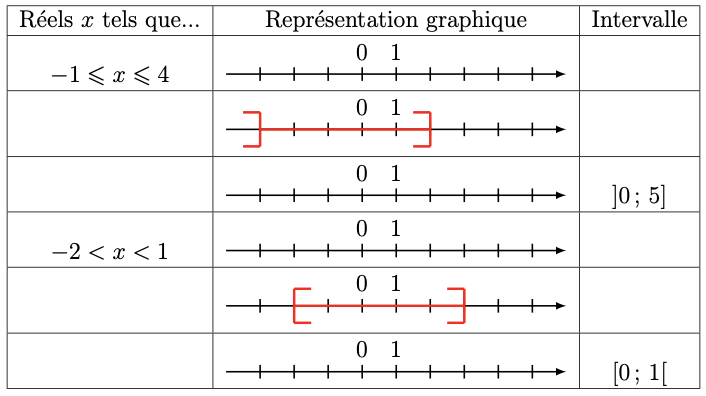
\includegraphics[scale=0.7]{IMG/Intervalle1.png}
\end{center}

\end{Exercice}



\begin{Exercice}
Compléter le tableau suivant selon le modèle vu dans la leçon.\\

\begin{center}
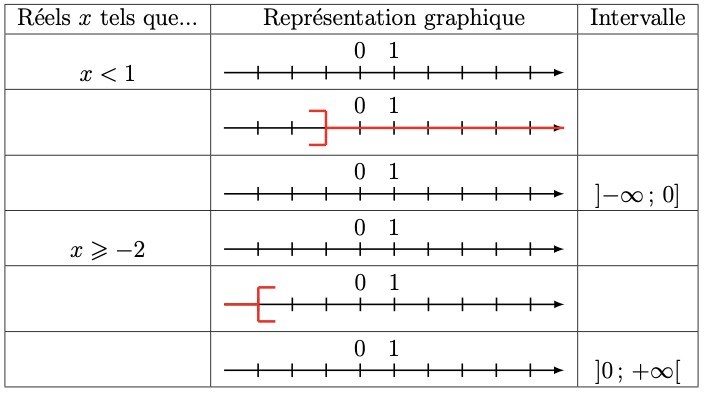
\includegraphics[scale=0.7]{IMG/Intervalle2.png}
\end{center}

\end{Exercice}

% @see : https://coopmaths.fr/alea?uuid=31c01&id=2N11-1&n=6&d=10&alea=sLrg&cd=1&cols=1
\begin{Exercice}
\leavevmode\vspace{-\baselineskip}
\begin{enumerate}[itemsep=1em]
	\item \begin{minipage}[t]{\linewidth}Déterminer l'inéquation correspondant à $x \in ]15;+\infty[$ et représenter l'intervalle sur une droite graduée.\end{minipage}
	\item \begin{minipage}[t]{\linewidth}Déterminer l'intervalle $I$ de $\mathbb{R}$ correspondant à l'inéquation $9< x\leqslant 23$ et représenter l'intervalle sur une droite graduée.\end{minipage}
	\item \begin{minipage}[t]{\linewidth}Déterminer l'intervalle $I$ de $\mathbb{R}$ correspondant à l'inéquation $2\leqslant x\leqslant 3$ et représenter l'intervalle sur une droite graduée.\end{minipage}
	\item \begin{minipage}[t]{\linewidth}Déterminer l'intervalle $I$ de $\mathbb{R}$ correspondant à l'inéquation $x\geqslant 11$ et représenter l'intervalle sur une droite graduée.\end{minipage}
	\item \begin{minipage}[t]{\linewidth}Déterminer l'intervalle $I$ de $\mathbb{R}$ correspondant à l'inéquation $x>6$ et représenter l'intervalle sur une droite graduée.\end{minipage}
	\item \begin{minipage}[t]{\linewidth}Déterminer l'intervalle $I$ de $\mathbb{R}$ correspondant à l'inéquation $x\leqslant 2$ et représenter l'intervalle sur une droite graduée.\end{minipage}
\end{enumerate}
\end{Exercice}


\newpage
\subsubsection*{Réunion et intersection d'intervalles}
% @see : https://coopmaths.fr/alea?uuid=e356a&id=can2N03&n=8&d=10&alea=A3yh&cd=1&cols=1
\begin{Exercice}
Donner une écriture simplifiée des ensembles suivants :
\vspace{-0.5cm}
\begin{multicols}{2}
\begin{enumerate}[itemsep=1em]
	\item 
        $]-4\,;\,-1[\,\cap \,] -7\,;\,2]$.
	\item $]-\infty\,;\, -2]\,\cap \,]-\infty\,;\,2[$.
	\item 
          $[ -23\,;\,-2[\,\cap \,[0\,;\,11]$.
	\item $]-\infty \,; \,5]\cap ]9\,;\,+\infty[$.

\end{enumerate}
\end{multicols}
\vspace{-0.5cm}
\end{Exercice}

% @see : https://coopmaths.fr/alea?uuid=bb947&id=can2N04&n=8&d=10&alea=53kF&cd=1&cols=1
\begin{Exercice}
Donner une écriture simplifiée des ensembles suivants :
\vspace{-0.5cm}
\begin{multicols}{2}
\begin{enumerate}[itemsep=1em]
	\item $]4\,;\,11]\cup ]-\infty \,; \,7[$.
	\item $[-24\,;\,13]\,\cup \,[ -30\,;\,-5[$.
	\item $] -3\,;\,+\infty[\,\cup \,[-6\,;\,0[$.
	\item $]-11\,;\,-6]\cup ]-\infty \,; \,-10[$.
\end{enumerate}
\end{multicols}
\vspace{-0.5cm}
\end{Exercice}









% @see : https://coopmaths.fr/alea?uuid=dc2a5&id=2N11-2&n=10&d=10&alea=rHB4&cd=1&cols=2
\begin{Exercice}
Donner, si possible une écriture simplifiée des ensembles suivants :
\begin{multicols}{2}
\begin{enumerate}[itemsep=1em]
	\item $I=[7;25]\cap[27;38]$
	\item $I=]5;10]\cup]17;+\infty[$
	\item $I=[2;9[\cap[18;+\infty[$
	\item $I=[15;36[\cap[32;57[$
	\item $I=[2;25[\cup[6;13[$
	\item $I=]8;12]\cup[25;28]$
	\item $I=[13;30[\cup[18;46[$
	\item $I=[11;33[\cap]21;22[$
	\item $I=]2;18]\cup]27;28]$
	\item $I=[6;7[\cap[15;+\infty[$
\end{enumerate}
\end{multicols}
\end{Exercice}



\subsection*{Puissances, notation scientifique et arrondis}
\subsubsection*{Puissances}

% @see : https://coopmaths.fr/alea?uuid=fb1a4&id=2N31-9&n=6&d=10&s=2&s2=3&s3=3&s4=3&alea=TJPD&cd=1&cols=1
\begin{Exercice}
Simplifier l'écriture en utilisant la notation puissance.
\vspace{-0.5cm}
\begin{multicols}{2}
\begin{enumerate}[itemsep=1em]
	\item \begin{minipage}[t]{\linewidth}$ \dfrac{1}{(-2)\times(-2)\times(-2)\times(-2)\times(-2)}$\end{minipage}
	\item \begin{minipage}[t]{\linewidth}$- 4\times4$\end{minipage}
	\item \begin{minipage}[t]{\linewidth}$- 6\times6\times6\times6\times6\times6\times6\times6$\end{minipage}
	\item \begin{minipage}[t]{\linewidth}{\small $ \dfrac{1}{(-7)\times(-7)\times(-7)\times(-7)\times(-7)\times(-7)\times(-7)}$}\end{minipage}
	\item \begin{minipage}[t]{\linewidth}$ \dfrac{1}{5\times5\times5\times5\times5\times5}$\end{minipage}
	\item \begin{minipage}[t]{\linewidth}$- (-6)\times(-6)\times(-6)\times(-6)\times(-6)\times(-6)$\end{minipage}
\end{enumerate}
\end{multicols}
\vspace{-0.5cm}
\end{Exercice}
\newpage
% @see : https://coopmaths.fr/alea?uuid=53fbb&id=2N31-0&n=12&d=10&s=true&s2=false&alea=IHDi&cd=1&cols=2
\begin{Exercice}
Calculer de tête l'écriture décimale ou fractionnaire des nombres suivants.
\vspace{-0.5cm}
\begin{multicols}{3}
\begin{enumerate}[itemsep=1em]
	\item \begin{minipage}[t]{\linewidth}$-25^{1} = $\end{minipage}
	\item \begin{minipage}[t]{\linewidth}$-2^{7} = $\end{minipage}
	\item \begin{minipage}[t]{\linewidth}$(-7)^{2} = $\end{minipage}
	\item \begin{minipage}[t]{\linewidth}$16^{0} = $\end{minipage}
	\item \begin{minipage}[t]{\linewidth}$-2^{2} = $\end{minipage}
	\item \begin{minipage}[t]{\linewidth}$(-4)^{3} = $\end{minipage}
	\item \begin{minipage}[t]{\linewidth}$(-2)^{-8} = $\end{minipage}
	\item \begin{minipage}[t]{\linewidth}$3^{-2} = $\end{minipage}
	\item \begin{minipage}[t]{\linewidth}$(-3)^{-3} = $\end{minipage}
	\item \begin{minipage}[t]{\linewidth}$2^{4} = $\end{minipage}
	\item \begin{minipage}[t]{\linewidth}$(-5)^{3} = $\end{minipage}
	\item \begin{minipage}[t]{\linewidth}$(-3)^{-2} = $\end{minipage}
\end{enumerate}
\end{multicols}
\vspace{-0.5cm}
\end{Exercice}
% @see : https://coopmaths.fr/alea?uuid=1e42b&id=2N31-2&n=12&d=10&s=5&s2=3&alea=Gagx&cd=0&cols=1



\begin{Exercice}
Écrire sous la forme $a^n$.
\vspace{-0.5cm}
\begin{multicols}{3}
\begin{enumerate}[itemsep=1em]
\item \begin{minipage}[t]{\linewidth}$A=((-2)^3)^{3}$\end{minipage}
	\item \begin{minipage}[t]{\linewidth}$B=(7^3)^{3}$\end{minipage}
	\item \begin{minipage}[t]{\linewidth}$C=3^5\times 5^5$\end{minipage}
	\item \begin{minipage}[t]{\linewidth}$D=\dfrac{8^3}{8^2}$\end{minipage}
	\item \begin{minipage}[t]{\linewidth}$E=((-2)^2)^{4}$\end{minipage}
	\item \begin{minipage}[t]{\linewidth}$F=\dfrac{2^4}{2^5}$\end{minipage}
	\item \begin{minipage}[t]{\linewidth}$G=5^3\times 8^3$\end{minipage}
	\item \begin{minipage}[t]{\linewidth}$H=3^3\times 3^4$\end{minipage}
	\item \begin{minipage}[t]{\linewidth}$I=(-8)^4\times (-8)^5$\end{minipage}
\end{enumerate}
\end{multicols}
\vspace{-0.5cm}
\end{Exercice}

% @see : https://coopmaths.fr/alea?uuid=c71da&id=2N31-3&n=12&d=10&alea=qofs&cd=1&cols=1
\begin{Exercice}
Écrire sous la forme $a^n$.
\vspace{-0.5cm}
\begin{multicols}{3}
\begin{enumerate}[itemsep=1em]
	\item \begin{minipage}[t]{\linewidth}$\dfrac{2^6\times 8}{2^2}$\end{minipage}
	\item \begin{minipage}[t]{\linewidth}$\dfrac{3^4\times 3^2}{9^2}\times 3$\end{minipage}
	\item \begin{minipage}[t]{\linewidth}$\dfrac{5\times 5^3}{25^2}$\end{minipage}
	\item \begin{minipage}[t]{\linewidth}$\dfrac{27^3}{3}$\end{minipage}
	\item \begin{minipage}[t]{\linewidth}$\dfrac{2\times 2^6}{4\times 4}$\end{minipage}
	\item \begin{minipage}[t]{\linewidth}$\dfrac{3^7\times 9}{3^4 \times 3^2}$\end{minipage}
	\item \begin{minipage}[t]{\linewidth}$\dfrac{4^3}{2}$\end{minipage}
	\item \begin{minipage}[t]{\linewidth}$\dfrac{8\times 2}{4^3}$\end{minipage}
	\item \begin{minipage}[t]{\linewidth}$\dfrac{27^2}{3}$\end{minipage}
\end{enumerate}
\end{multicols}
\vspace{-0.5cm}
\end{Exercice}



% @see : https://coopmaths.fr/alea?uuid=816c8&id=2N31-6&n=10&d=10&s=3&s2=3&s3=3&alea=TS6A&cd=1&cols=1


\begin{Exercice}
Écrire sous la forme $a^n$.
\vspace{-0.5cm}
\begin{multicols}{3}
\begin{enumerate}[itemsep=1em]
	\item \begin{minipage}[t]{\linewidth}$x^{5}\times x^{3}$\end{minipage}
	\item \begin{minipage}[t]{\linewidth}$x^{6}\times x^{-2}$\end{minipage}
	\item \begin{minipage}[t]{\linewidth}$\dfrac{x^{9}}{x^{3}}$\end{minipage}
	\item \begin{minipage}[t]{\linewidth}$\dfrac{x^{-2}}{x^{5}}$\end{minipage}
	\item \begin{minipage}[t]{\linewidth}$x^3\times x^7\times x^{-4}$\end{minipage}
	\item \begin{minipage}[t]{\linewidth}$\dfrac{x^2\times x^5{-1}}{x^4\times x^3}$\end{minipage}
	\item \begin{minipage}[t]{\linewidth}$(x^3\times x^2)^4$\end{minipage}
	\item \begin{minipage}[t]{\linewidth}$((x^2)^6)^3$\end{minipage}
	\item \begin{minipage}[t]{\linewidth}$\left(\dfrac{x^3\times x}{x^{-2}\times(x^3)^{-1}}\right)^2$\end{minipage}
\end{enumerate}
\end{multicols}
\vspace{-0.5cm}
\end{Exercice}
\newpage

\subsubsection*{Notation scientifique}


\begin{Exercice}
Donner la notation scientifique des nombres suivants.
\vspace{-0.5cm}
\begin{multicols}{3}
\begin{enumerate}[itemsep=1em]
	\item \begin{minipage}[t]{\linewidth}$0{,}005\,01 \times 10^{7}$\end{minipage}
	\item \begin{minipage}[t]{\linewidth}$0{,}531 \times 10^{-6}$\end{minipage}
	\item \begin{minipage}[t]{\linewidth}$8\,680 \times 10^{-8}$\end{minipage}
	\item \begin{minipage}[t]{\linewidth}$0{,}068\,4 \times 10^{5}$\end{minipage}
	\item \begin{minipage}[t]{\linewidth}$0{,}060\,3 \times 10^{-7}$\end{minipage}
	\item \begin{minipage}[t]{\linewidth}$0{,}307 \times 10^{-9}$\end{minipage}
	\item \begin{minipage}[t]{\linewidth}$0{,}888 \times 10^{-6}$\end{minipage}
	\item \begin{minipage}[t]{\linewidth}$156 \times 10^{7}$\end{minipage}
	\item \begin{minipage}[t]{\linewidth}$0{,}005\,07 \times 10^{10}$\end{minipage}
	\item \begin{minipage}[t]{\linewidth}$2\,030 \times 10^{9}$\end{minipage}
\end{enumerate}
\end{multicols}
\vspace{-0.5cm}
\end{Exercice}


\subsection*{Équations et inéquations}
\subsubsection*{Équations de degré 1}
% @see : https://coopmaths.fr/alea?uuid=f239f&id=3L13&n=6&d=10&s=true&s2=8&s3=true&alea=7tmd&cd=1&cols=1
\begin{Exercice}
Résoudre les équations suivantes.
\leavevmode\vspace{-\baselineskip}
\begin{multicols}{3}
\begin{enumerate}[itemsep=1em]
	\item \begin{minipage}[t]{\linewidth}$x+1=1$\end{minipage}
	\item \begin{minipage}[t]{\linewidth}$\dfrac{3x}{-7}=-3$\end{minipage}
	\item \begin{minipage}[t]{\linewidth}$11x-13=0$\end{minipage}
	\item \begin{minipage}[t]{\linewidth}$12x-4=-13x-10$\end{minipage}
	\item \begin{minipage}[t]{\linewidth}$-3x+6=1$\end{minipage}
	\item \begin{minipage}[t]{\linewidth}$\dfrac{x}{-8}=6$\end{minipage}
\end{enumerate}
\end{multicols}
\end{Exercice}

% @see : https://coopmaths.fr/alea?uuid=1802d&id=3L13-1&n=4&d=10&alea=RTKt&cd=1&cols=1
\begin{Exercice}
Résoudre les équations suivantes.
\leavevmode\vspace{-\baselineskip}
\begin{multicols}{2}
\begin{enumerate}[itemsep=1em]
	\item \begin{minipage}[t]{\linewidth}$4-(-3x-3)=-8x-5$\\\end{minipage}
	\item \begin{minipage}[t]{\linewidth}$6(7x-6)=9x-3$\\\end{minipage}
	\item \begin{minipage}[t]{\linewidth}$11x+3=5x+3$\\\end{minipage}
	\item \begin{minipage}[t]{\linewidth}$15x+4=9x-7$\\\end{minipage}
\end{enumerate}
\end{multicols}
\end{Exercice}



% @see : https://coopmaths.fr/alea?uuid=22412&id=3L13-3&n=7&d=10&s=1-3-4-5-9-10-11&s2=false&alea=OsKZ&cd=1&cols=1
\begin{Exercice}
\leavevmode\vspace{-\baselineskip}
\begin{enumerate}[itemsep=1em]
	\item \begin{minipage}[t]{\linewidth}Un quadrilatère possède un côté de longueur $2{,}6$ cm et tous ses autres côtés ont même longueur.\\Son périmètre est $38$ cm.\\Quelle est la longueur des côtés de même longueur ?\end{minipage}
	\item \begin{minipage}[t]{\linewidth}Un triangle isocèle a pour périmètre $260$ mm. Sa base est plus petite que les côtés égaux de $13$ mm.\\Quelle est la mesure de sa base ? (La figure n'est pas en vraie grandeur.)\\
	\begin{center}
	\begin{tikzpicture}[baseline,scale = 0.8]

    \tikzset{
      point/.style={
        thick,
        draw,
        cross out,
        inner sep=0pt,
        minimum width=5pt,
        minimum height=5pt,
      },
    }
    \clip (-1,-1) rectangle (7,4);
    	\draw[color={black}] (6,1.5)--(0,3)--(0,0)--cycle;
	\draw [color={black}] (3,2.25) node[anchor = center,scale=1, rotate = -15] {//};
\draw [color={black}] (3,0.75) node[anchor = center,scale=1, rotate = -345] {//};


\end{tikzpicture}
	\end{center}\end{minipage}
	\item \begin{minipage}[t]{\linewidth}Christophe et Teresa choisissent un même nombre.\\ Christophe lui ajoute 6 puis multiplie le résultat par 12 alors que Teresa lui ajoute 5 puis multiplie le résultat par 14.\\Christophe et Teresa obtiennent le même résultat.\\Quel nombre commun ont choisi Christophe et Teresa ?\end{minipage}
	\item \begin{minipage}[t]{\linewidth}Dans une salle de spectacle de $2\,830$ places, le prix d'entrée pour un adulte est $11{,}20$€~et pour un enfant il est de $7{,}60$€.\\Le spectacle de ce soir s'est déroulé devant une salle pleine et la recette est de $27\,390{,}40$€.\\Combien d'adultes y avait-il dans la salle ?\end{minipage}
	\item \begin{minipage}[t]{\linewidth}Une équipe de basket a marqué 93 points lors d'un match. Au cours de ce match, elle a marqué 28 points sur lancers francs.\\L'équipe a marqué 5 paniers à deux points de plus que de paniers à trois points.\\Combien a-t-elle marqué de paniers à trois points ?\end{minipage}
	\item \begin{minipage}[t]{\linewidth}Le club de fitness d'un village propose deux tarifs à ses pratiquants.\\Le tarif A propose de payer $5{,}80$€~à chaque séance.\\Le tarif B propose de payer un abonnement annuel de $30$€~puis de payer $4{,}30$€~par séance.\\Pour quel nombre de séances le tarif B devient-il plus avantageux que le tarif A ?\end{minipage}
	\item \begin{minipage}[t]{\linewidth}Yasmine a acheté $4{,}4$ kg de citrons avec un billet de $10$€. Le marchand lui a rendu $1{,}20$€.\\Quel est le prix d'un kilogramme de citrons ?\end{minipage}
\end{enumerate}
\end{Exercice}



\subsubsection*{Inéquations de degré 1}

% @see : https://coopmaths.fr/alea?uuid=bc1e4&id=2N60-4&n=12&d=10&s=true&s2=4&alea=QIq4&cd=1&cols=1
\begin{Exercice}
Résoudre les inéquations suivantes.
\leavevmode\vspace{-\baselineskip}
\begin{multicols}{3}
\begin{enumerate}[itemsep=1.5em]
	\item \begin{minipage}[t]{\linewidth}$2x\geqslant4$\\\end{minipage}
	\item \begin{minipage}[t]{\linewidth}$10x-2<-5$\\\end{minipage}
	\item \begin{minipage}[t]{\linewidth}$6x+7< -11x+5$\\\end{minipage}
	\item \begin{minipage}[t]{\linewidth}$x-6<11$\\\end{minipage}
	\item \begin{minipage}[t]{\linewidth}$-13x+10\leqslant0$\\\end{minipage}
	\item \begin{minipage}[t]{\linewidth}$-10x+7\leqslant0$\\\end{minipage}
	\item \begin{minipage}[t]{\linewidth}$-10x-13\geqslant -6x-11$\\\end{minipage}
	\item \begin{minipage}[t]{\linewidth}$11x+11\leqslant-6$\\\end{minipage}
	\item \begin{minipage}[t]{\linewidth}$-8x>-6$\\\end{minipage}
	\item \begin{minipage}[t]{\linewidth}$x+13<9$\\\end{minipage}
	\item \begin{minipage}[t]{\linewidth}$-7x\geqslant6$\\\end{minipage}
	\item \begin{minipage}[t]{\linewidth}$-9x+11>0$\\\end{minipage}
\end{enumerate}
\end{multicols}
\end{Exercice}

% @see : https://coopmaths.fr/alea?uuid=d2084&id=2N60-1&n=5&d=10&s=4&alea=u4Ip&cd=1&cols=1
\begin{Exercice}
\leavevmode\vspace{-\baselineskip}
\begin{enumerate}[itemsep=1.5em]
	\item $ $ \begin{minipage}[c]{0.6\linewidth} Soit $ABCD$ un rectangle tel que $AD=8$ et $DC=17$.\\
            $M$ est un point du segment $[AB]$. On note $AM=x$.\\
            Pour quelles valeurs de $x$ l'aire du triangle $AMD$ est-elle au plus égale au cinquième de l'aire du triangle $CMB$ ? \end{minipage} \hfill \begin{minipage}[c]{0.4\linewidth}
     \begin{center}

              \begin{tikzpicture}[baseline,scale = 0.5]

    \tikzset{
      point/.style={
        thick,
        draw,
        cross out,
        inner sep=0pt,
        minimum width=5pt,
        minimum height=5pt,
      },
    }
    \clip (-1,-1) rectangle (12,8);
    	\draw[color ={Couleur6}] (0,0)--(10,0);
	\draw[color ={Couleur6}] (10,0)--(10,6);
	\draw[color ={Couleur6}] (0,6)--(0,0);
	\draw[color ={Couleur6}] (10,6)--(0,6);
	\draw [color={black}] (0,-0.5) node[anchor = center,scale=1, rotate = 0] {A};
	\draw [color={black}] (10,-0.5) node[anchor = center,scale=1, rotate = 0] {B};
	\draw [color={black}] (10,6.5) node[anchor = center,scale=1, rotate = 0] {C};
	\draw [color={black}] (0,6.5) node[anchor = center,scale=1, rotate = 0] {D};
	\draw [color={black}] (4,-0.5) node[anchor = center,scale=1, rotate = 0] {M};
	\draw[color={Couleur6},preaction={fill,color = {Couleur6!40}}] (0,0)--(4,0)--(0,6)--cycle;
	\draw[color={Couleur6},preaction={fill,color = {Couleur6!40}}] (10,6)--(4,0)--(10,0)--cycle;
	\draw [color={black}] (2,-0.7) node[anchor = center,scale=1, rotate = 0] {$ x $};
	\draw [color={black}] (-0.5,3) node[anchor = center,scale=1, rotate = 0] {$ 8 $};
	\draw [color={black}] (5,6.5) node[anchor = center,scale=1, rotate = 0] {$ 17 $};

\end{tikzpicture}
     \end{center}\end{minipage}
	\item \begin{minipage}[t]{\linewidth} Pour la location mensuelle d'un véhicule, une entreprise propose le tarif suivant :\\
            Forfait de $101$€~quelque soit le nombre de km parcourus, puis un supplément par kilomètre parcouru de $0{,}22$€. \\
            
            Elsa loue une voiture à cette société. Elle a un budget de $280$€~et ne veut pas le dépasser.\\
                      Quel est le nombre maximum de km (arrondi à l'unité si besoin) qu'elle pourra parcourir sans dépasser son budget ?
                                   \\\end{minipage}
	\item \begin{minipage}[t]{\linewidth} \textbf{Voici un programme de calcul :} 	\begin{itemize}[label=\textcolor{Couleur6}{$\bullet$}]
		\item Choisir un nombre
		\item Multiplier ce nombre par $-4$
		\item Ajouter $8$
		\item Multiplier le résultat par $3$
	\end{itemize}Quels nombres doit-on choisir au départ pour obtenir un nombre strictement supérieur à $-20$.

\medskip
\end{minipage}
	\item \begin{minipage}[t]{\linewidth} On considère la figure ci-dessous sur laquelle les longueurs sont en cm. \\
            Quelles sont les valeurs possibles de $x$ pour que l'aire de cette  figure dépasse  $58$ cm$^2$ ?\\
            Résoudre ce problème en le modélisant par une inéquation.\\
             \begin{center}
              \begin{tikzpicture}[baseline,scale = 0.5]

    \tikzset{
      point/.style={
        thick,
        draw,
        cross out,
        inner sep=0pt,
        minimum width=5pt,
        minimum height=5pt,
      },
    }
    \clip (-3,-1) rectangle (12,9);
    	\draw[color={Couleur6}] (0,0)--(8,0)--(8,2)--(0,2)--cycle;
	\draw[color={Couleur6}] (8,0)--(10,0)--(10,2)--(8,2)--cycle;
	\draw[color={Couleur6}] (0,2)--(8,2)--(4,8)--cycle;
	\draw[color ={Couleur6}, densely dash dot dot ] (4,8)--(4,2);
	\draw[color={Couleur6},line width = 0.5] (4,2)--(4,2.4)--(4.4,2.4)--(4.4,2)--cycle;
	\draw [color={black}] (4,-0.6) node[anchor = center,scale=1, rotate = 0] {$ x $};
	\draw [color={black}] (-0.8,1) node[anchor = center,scale=1, rotate = 0] {$ 2 $};
	\draw [color={black}] (9,-0.6) node[anchor = center,scale=1, rotate = 0] {$ 2 $};
	\draw [color={black}] (4.5,5) node[anchor = center,scale=1, rotate = 0] {$ 8 $};

\end{tikzpicture}
             \end{center}\end{minipage}


	\item On considère la figure ci-dessous (l'unité est le centimètre). \\
            Quelles sont les valeurs possibles de $x$ pour que le périmètre de la figure soit supérieur à $59$ cm.\\
              \begin{center}
              \begin{tikzpicture}[baseline,scale = 0.5]

    \tikzset{
      point/.style={
        thick,
        draw,
        cross out,
        inner sep=0pt,
        minimum width=5pt,
        minimum height=5pt,
      },
    }
    \clip (-3,-1) rectangle (12,8);
    	\draw[color={Couleur6}] (0,0)--(10,0)--(10,6)--(0,6)--(0,2)--(-2,2)--(-2,0)--cycle;
	\draw[color ={Couleur6}, densely dash dot dot ] (0,0)--(0,2);
	\draw [color={black}] (-2.5,1) node[anchor = center,scale=1, rotate = 0] {$ x $};
	\draw [color={black}] (-1,-0.5) node[anchor = center,scale=1, rotate = 0] {$ x $};
	\draw [color={black}] (11,3) node[anchor = center,scale=1, rotate = 90] {$ x +6 $};
	\draw [color={black}] (5,-0.5) node[anchor = center,scale=1, rotate = 0] {$ 12 $};

\end{tikzpicture}
              \end{center}
\end{enumerate}
\end{Exercice}
}
